% \documentclass[fleqn,10pt,serif,xcolor=svgnames,xcolor=table,aspectratio=169]{beamer}
\documentclass[fleqn,10pt,serif,xcolor=svgnames,xcolor=table,aspectratio=169]{beamer}
% \includeonlyframes{current}
%========================================
% Packages
%========================================

\usepackage[palatino]{../../99-auxiliary-files/00-mypackBeamer}
\usepackage{../../99-auxiliary-files/00-mycommands}
\usepackage{../../99-auxiliary-files/00-myenvironments-beamer}

\usepackage{tikz-qtree}
\usepackage{array}
\usepackage[absolute,overlay]{textpos}
\usepackage{ulem}

\usepackage{pgfplots}

%========================================
% More Layout (Beamer Special)
%========================================

\DefineNamedColor{named}{mycol}{cmyk}{0.6,0.6,0,0}
% \DefineNamedColor{named}{mygray}{cmyk}{0.05,0.05,0.05,0.05}
% \DefineNamedColor{named}{mygraylight}{cmyk}{0.017,0.017,0.017,0.017}

\definecolor{signal1}{rgb}{0.69, 0.25, 0.21}
\definecolor{signal2}{rgb}{1.0, 0.66, 0.07}
\definecolor{signal3}{rgb}{0.39, 0.58, 0.93}
\definecolor{signal4}{rgb}{0.0, 0.4, 0.0}
\definecolor{firebrick}{rgb}{0.7, 0.13, 0.13}
\definecolor{themecolor}{rgb}{0.3, 0.36, 0.33} % feldgrau
\definecolor{darkgray}{rgb}{0.66, 0.66, 0.66}

% \usetheme[height=7mm]{Rochester}
%\usetheme{Warsaw}


\usecolortheme{dove}

% \useoutertheme[compress,subsection=false]{miniframes}

\usecolortheme[named=themecolor]{structure}

\setbeamercolor{title}{fg=themecolor}

% \setbeamercolor{lower separation line head}{bg=white}

%\setbeamercolor{structure}{fg=Brown}
%\setbeamercolor{normal text}{fg=Brown}
%\setbeamercolor{section in head/foot}{bg=gray!40}
%%\setbeamercolor{lower separation line head}{bg=black!40}
%\setbeamercolor*{frametitle}{fg=Black,bg=gray!40}
%\setbeamercolor*{block body}{fg=Brown,bg=gray!00}
%\setbeamercolor*{block title}{fg=Black,bg=gray!40}


% Switch of shadows of boxes
\setbeamertemplate{blocks}[default]

% Frame numbers in footer
\setbeamertemplate{footline}[frame number]

% See-through preview for uncovered
% \setbeamercovered{transparent}

% Switch off navigation panel at bottom right
\beamertemplatenavigationsymbolsempty

% Change Style for itemize markers
% Options are ball, circle, rectangle and default (=triangle)
\setbeamertemplate{items}[circle]



\setcounter{tocdepth}{1}

% Use bullets in enumerates and TOC
\setbeamertemplate{enumerate item}[circle]

% Set color for enumerate/TOC bullets to white
\setbeamercolor*{item projected}{fg=themecolor,bg=gray!00}

\setbeamercolor*{author}{fg=gray!80}

\setbeamerfont*{block title}{size=\normalsize}
\setbeamerfont*{title}{size=\huge}
\setbeamerfont*{subtitle}{size=\large}

% \newcommand{\mygray}[1]{{\color{gray}{#1}}}
% \newcommand{\mycol}[1]{{\color{mycol}{#1}}}

\newcommand{\mycomment}[1]{\hfill {\mygray{#1}}}
\newcommand{\mycom}[1]{\hfill {\mygray{[#1]}}}

\newcommand{\slideFN}[1]{%
  \begin{textblock*}{\paperwidth}(0pt,1.05\textheight)
    \hfill \footnotesize{\mygray{#1}} \hspace{.5em}
  \end{textblock*}}

\newcommand{\pictureslide}[2][current]{
\usebackgroundtemplate{\includegraphics[width=\paperwidth]{#2}}%
\begin{frame}[label=#1]

\end{frame}
}
% code below makes it possible to turn inclusion of frames
% into 'miniframes' off and on with commands:
% \miniframeson and \miniframesoff
% from: http://tex.stackexchange.com/questions/37127/how-to-remove-some-pages-from-the-navigation-bullets-in-beamer

\makeatletter
\let\beamer@writeslidentry@miniframeson=\beamer@writeslidentry
\def\beamer@writeslidentry@miniframesoff{%
  \expandafter\beamer@ifempty\expandafter{\beamer@framestartpage}{}% does not happen normally
  {%else
    % removed \addtocontents commands
    \clearpage\beamer@notesactions%
  }
}
\newcommand*{\miniframeson}{\let\beamer@writeslidentry=\beamer@writeslidentry@miniframeson}
\newcommand*{\miniframesoff}{\let\beamer@writeslidentry=\beamer@writeslidentry@miniframesoff}
\makeatother

\setbeamertemplate{bibliography item}{}


%========================================
% Commands
%========================================

\newcommand{\mycol}[1]{{\textcolor{mycol}{#1}}}
\renewcommand{\markdef}[1]{\textcolor{themecolor}{\textbf{#1}}}
\newcommand{\mygray}[1]{\textcolor{gray}{#1}}
\definecolor{darkgray}{rgb}{0.66, 0.66, 0.66}

\renewcommand{\slideFN}[1]{%
  \begin{textblock*}{\paperwidth}(0pt,0.95\textheight)
    \hfill \footnotesize{\mygray{#1}} \hspace{.5em}
  \end{textblock*}}

\newcommand{\proplog}{\acro{PropLog}}
\newcommand{\predlog}{\acro{PredLog}}

\newcommand{\mult}{\ensuremath{\cdot}}
\def\checkmark{\tikz\fill[scale=0.4](0,.35) -- (.25,0) -- (1,.7) -- (.25,.15) -- cycle;}

%========================================
% Document
%========================================

\title{Methods 1: Logic}
\subtitle{Introduction, overview, \& practicalities}

\author{Michael Franke}
\date{}


%--------------------------------------

\begin{document}

% --- Horizontal Space Fix ----

\abovedisplayskip=3pt
\abovedisplayshortskip=3pt

\belowdisplayskip=3pt
\belowdisplayshortskip=3pt

\begin{frame}
  \maketitle
\end{frame}

\begin{frame}
  \begin{center}
    \begin{Huge}
      Why are you here?
    \end{Huge}
  \end{center}
\end{frame}

\begin{frame}
  \frametitle{Reasoning: fast \& slow}

  A baseball bat and a ball cost \$11.\\
  The bat is \$10 more than the ball.

  \medskip

  How much is the bat? How much is the ball?

\end{frame}

\begin{frame}
  \frametitle{Logic puzzle}

  There are two villages.
  In the honest village ($H$) everybody always speaks the truth.
  In the dishonest village ($D$) everybody always says the opposite of what is true.

  Before you the road splits: one way leads to the honest, the other to the dishonest village.
  At the splitting there is a man.
  He may be from village $H$ or $D$, you don't know.

  What do you ask the man to find out where the honest village is?

  \bigskip \pause

  \begin{center}
    \begin{tabular}{>{\columncolor{olive!15}}cc>{\columncolor{olive!15}}c}
      honest village & man       & where're you from? \\ \midrule
      left           & honest    & ``left'' \\
      left           & dishonest & ``left'' \\
      right          & honest    & ``right''\\
      right          & dishonest & ``right''
    \end{tabular}
  \end{center}

\end{frame}

\newcolumntype{C}[1]{>{\centering\arraybackslash}p{#1}}

\begin{frame}
  \frametitle{What is logic?}

  \begin{center}
    \begin{Large}
      \begin{tabular}{C{2cm}C{4cm}C{2cm}}
        proof & entailment & meaning
      \end{tabular}
    \end{Large}
  \end{center}

  \pause
  \bigskip

  \begin{center}
    All Europeans are human.\\
    All humans are mortal\\
    Therefore, all Europeans are mortal.
  \end{center}
\end{frame}

\begin{frame}
  \frametitle{Modeling}

  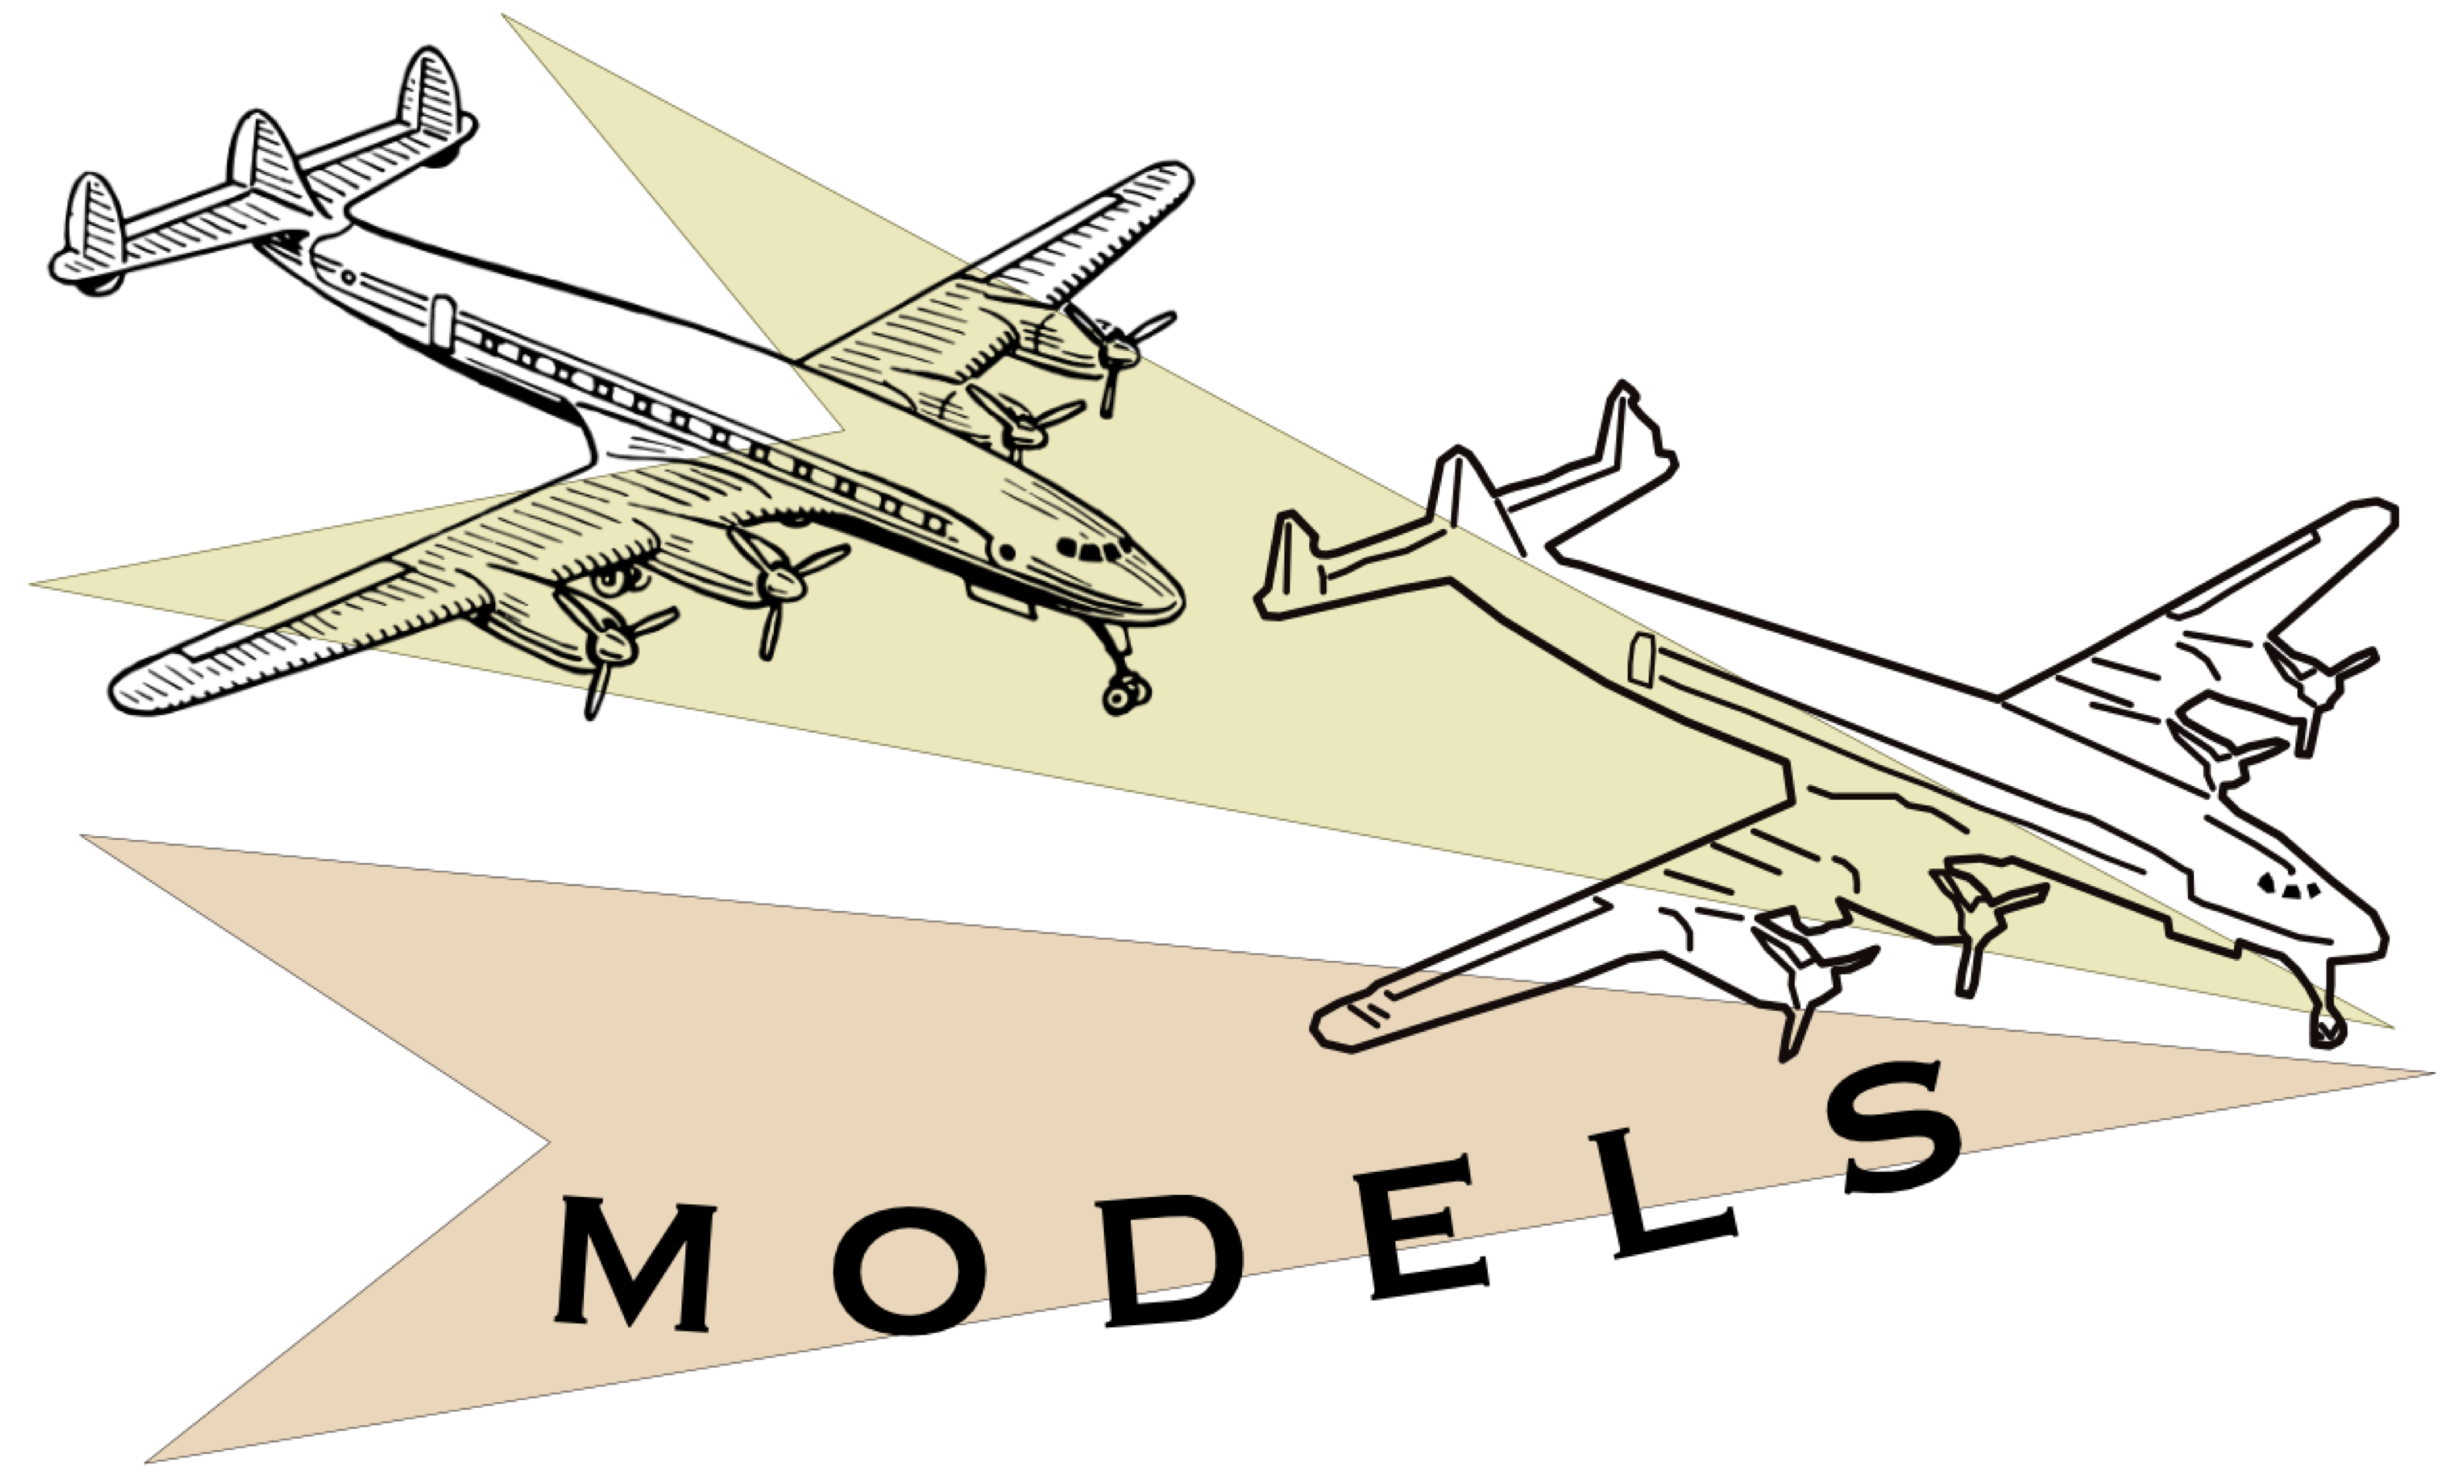
\includegraphics[width=0.9\textwidth]{00-introduction-pics/model-planes.png}

\end{frame}

\begin{frame}
  \frametitle{Logic as a \textit{normative} model: how language \& thought \textit{should} be}

  \begin{center}
    \begin{Large}
      \begin{tabular}{C{4cm}C{4cm}C{4cm}}
        proof & entailment & meaning \\
              & \\
        argumentation & inference & precision of expression
      \end{tabular}
    \end{Large}
  \end{center}


  \bigskip

  \begin{center}
    \begin{footnotesize}
      \mygray{The focus of this course is more on logic as a tool in psychological / linguistic explanations. There will be less emphasis on the role of logic in the foundations of mathematics (so-called logicism).}
    \end{footnotesize}
  \end{center}


\end{frame}

\begin{frame}
  \frametitle{Big-picture learning goals}
  \begin{itemize}
    \item understand the significance of logic for the development of modern Linguistics, Philosophy, Cognitive Science and AI
    \begin{itemize}
      \item formal language theory (with syntax \& semantics); meta vs object language
      \item picture theory of meaning and correspondence theory of truth
      \item symbol-manipulation theory of human cognition
    \end{itemize}
    \item distinguish ``good reasoning'' from ``fallacious reasoning'', as well as ``logical entailment'' from ``commonsense entailment''
    \item be able to excavate the logical structure of natural language sentences and represent it in logical notation
  \end{itemize}
\end{frame}

\begin{frame}
  \frametitle{What is \textbf{a} logic?}

  \begin{itemize}
    \item there are different kinds of logic
    \item a logic is a formal system that captures some structural properties of meaning
    \item this course will cover three logics:
    \begin{enumerate}
      \item propositional logic \mycom{meaning of connectives \textit{and}, \textit{or}, \textit{not} \dots}
      \item predicate logic \mycom{meaning of quantifiers \textit{all}, \textit{some}, \textit{none} \dots}
      \item modal logic \mycom{meaning of epistemic attitudes \textit{belief}, \textit{knowledge} \dots}
    \end{enumerate}
  \end{itemize}

\end{frame}

\begin{frame}
  \frametitle{Course content}

  \begin{minipage}{0.42\linewidth}

    \begin{itemize}
      \item set theory
      \item (informal) proofs
      \item propositional logic
      \item predicate logic
      \item natural deduction
      \item modal (epistemic) logic
      \item probability theory
      \item information theory
    \end{itemize}
  \end{minipage}
  %
  \hfill
  %
  \begin{minipage}{0.57\linewidth}
    \begin{tabular}{rlll}
          & topic\\ \midrule
      1   & Course overview \      \\%& introduction\\
      2   & Basics of (naive) set theory\\
      3   & Proofs\\
      4   & Relations \            \\%& functions\\
      5   & PropLog: Syntax \      \\%& truth tables\\
      6   & PropLog: Translations \& logical validity\\
      7   & Natural Deduction (PropLog) \\
      8   & PredLog: Syntax \      \\%& Translations\\
      9   & PredLog: Semantics \   \\%& Identity\\ %\midrule
      10  & Modal logic\\
      11  & Probability theory\\
      12  & Information theory\\
      13  & Recap\\
      14  & Final exam\\
    \end{tabular}
  \end{minipage}
\end{frame}



\begin{frame}
  \frametitle{Practicalities}
  \begin{itemize}
    \item enroll for this course on \textbf{moodle}
    \item necessary for
    \begin{itemize}
      \item assessing course material
      \item receiving notifications
      \item asking questions in the forum
      \item submitting homework
      \item receiving feedback on homework
    \end{itemize}
  \end{itemize}
\end{frame}

\begin{frame}
  \frametitle{Best practice guide}
  \begin{enumerate}
    \item self-study
    \begin{itemize}
      \item prepare the assigned reading material \emph{before} the lecture
      \item bring questions, know what you don't know, ask and probe
    \end{itemize}
    \item lecture
    \begin{itemize}
      \item provides motivation, context and overview
      \item focuses on conceptual understanding
    \end{itemize}
    \item homework \hfill \mycom{start as early as possible each week}
    \begin{itemize}
      \item discussion with others is allowed \& encouraged
      \item write-up \& submissions must be made individually
      \item ask general questions on moodle, but do not share solutions
    \end{itemize}
    \item tutorials \hfill \mycom{go to at least one tutorial every week!}
    \begin{itemize}
      \item start working on homework questions \emph{before} the tutorial(s)
      \item emphasis on hands-on support for exercises
    \end{itemize}
  \end{enumerate}
\end{frame}


\begin{frame}

  \begin{center}
    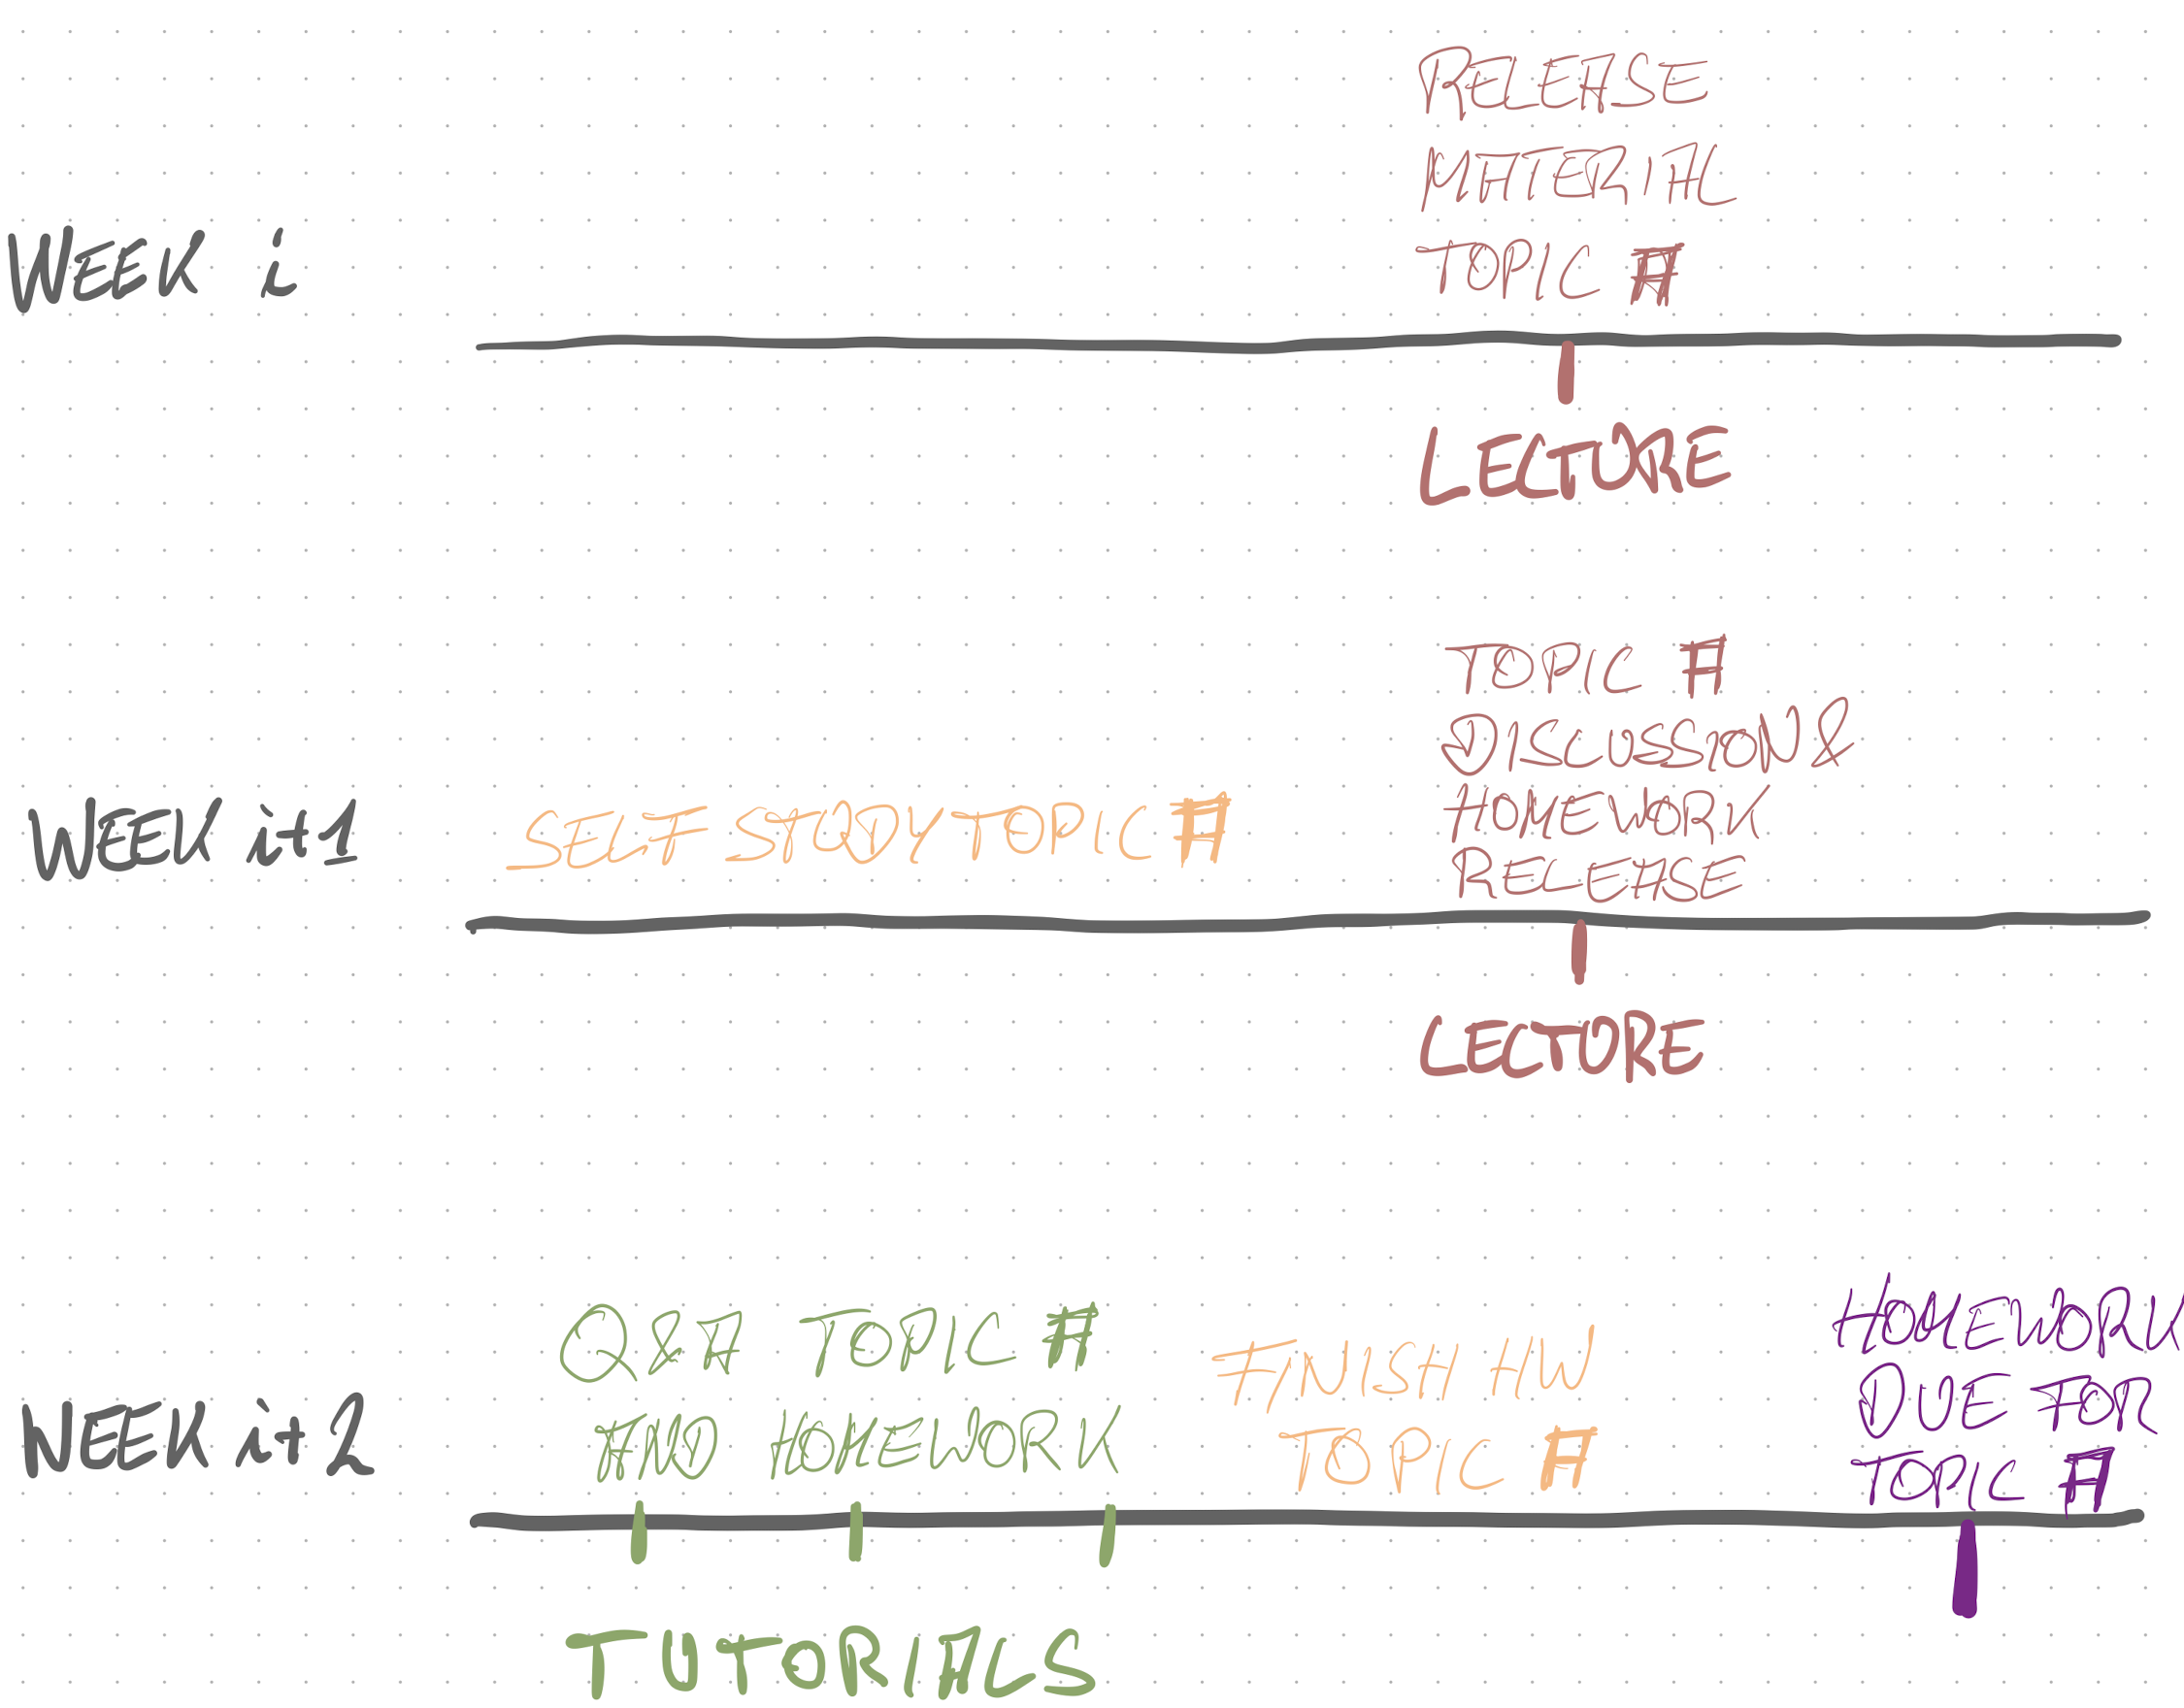
\includegraphics[width=0.75\textwidth]{00-introduction-pics/timing-logic.png}
  \end{center}

\end{frame}

\begin{frame}
  \frametitle{Tutorials}
  \begin{itemize}
    \item four different slots: \hfill \mycom{tutorials start in the week of Oct 28}
    \begin{enumerate}
      \item \makebox[11.5em][l]{Aida Rostami: }          Monday 12:00
      \item \makebox[11.5em][l]{Seoha Lee:  }            Thursday 12:00
      \item \makebox[11.5em][l]{Eric Zeiner: }           Thursday 16:00
      \item \makebox[11.5em][l]{Shanshan Xu: }           Friday 14:00
    \end{enumerate}
    \item sign up for your favorite slot on moodle!
    \item information on rooms on alma
  \end{itemize}
\end{frame}

\begin{frame}
  \frametitle{How to get answers}
  \begin{itemize}
    \item general questions (for everyone to see) about content:
    \begin{itemize}
      \item use the ``General Questions'' section on moodle
    % \item joing the dischord server: https://discord.gg/fJ7ZmZHw \\
    % 
\includegraphics[width=0.25\textwidth]{00-introduction-pics/qr-code.png}
    \end{itemize}
    \item confidential, non-content-related questions:
    \begin{itemize}
      \item email to lecturer \hfill \textcolor{orange}{do not use moodle's messaging system!!}
    \end{itemize}
  \end{itemize}
\end{frame}

\begin{frame}
  \frametitle{Homework}
  \begin{itemize}
    \item \textbf{no copying from others} \hfill \mycom{plagiarism will lead to failure}
    \item release: after the lecture
    \item submission due before that lecture (14:00 sharp)
    \begin{itemize}
      \item zero-tolerance on late submissions (see moodle)
    \end{itemize}
  \end{itemize}
\end{frame}

\begin{frame}
  \frametitle{Exam}
  \begin{itemize}
    \item February 4 2025, 14:00-16:00 (CET)
    \item open-book, in-class exam:
    \begin{itemize}
      \item solvable in ca.~90 minutes
      \item you may use any material you like (books, handouts, \dots)
      \item no cooperation, communication or any electronic devices
    \end{itemize}
  \end{itemize}
\end{frame}

\begin{frame}
  \frametitle{Homework}

  \begin{itemize}
    \item sign up for course on moodle
    \item sign up for preferred tutorial slot
    \item read section ``Course overview \& practicalities'' on moodle
    \item follow instructions in section ``Basics of (naive) set theory'' on moodle
    \begin{itemize}
      \item read handout
      \item watch videos
      \item try solving exercises in handout
      \item collect what you do not understand
    \end{itemize}
  \end{itemize}

\end{frame}

\end{document}
